%%%%%%%%%%%%%%%%%%%%%%%%%%%%%%%%%%%%%%%%%
% Beamer Presentation
% LaTeX Template
% Version 1.0 (10/11/12)
%
% This template has been downloaded from:
% http://www.LaTeXTemplates.com
%
% License:
% CC BY-NC-SA 3.0 (http://creativecommons.org/licenses/by-nc-sa/3.0/)
%
%%%%%%%%%%%%%%%%%%%%%%%%%%%%%%%%%%%%%%%%%

%----------------------------------------------------------------------------------------
%	PACKAGES AND THEMES
%----------------------------------------------------------------------------------------

\documentclass{beamer}

\mode<presentation> {

% The Beamer class comes with a number of default slide themes
% which change the colors and layouts of slides. Below this is a list
% of all the themes, uncomment each in turn to see what they look like.

%\usetheme{default}
%\usetheme{AnnArbor}
%\usetheme{Antibes}
%\usetheme{Bergen}
%\usetheme{Berkeley}
%\usetheme{Berlin}
%\usetheme{Boadilla}
%\usetheme{CambridgeUS}
%\usetheme{Copenhagen}
%\usetheme{Darmstadt}
%\usetheme{Dresden}
%\usetheme{Frankfurt}
%\usetheme{Goettingen}
%\usetheme{Hannover}
%\usetheme{Ilmenau}
%\usetheme{JuanLesPins}
%\usetheme{Luebeck}
\usetheme{Madrid}
%\usetheme{Malmoe}
%\usetheme{Marburg}
%\usetheme{Montpellier}
%\usetheme{PaloAlto}
%\usetheme{Pittsburgh}
%\usetheme{Rochester}
%\usetheme{Singapore}
%\usetheme{Szeged}
%\usetheme{Warsaw}

%%%%%%%%%%%%%%%%%%%%%%%%%%%%%
%REMOVE SLIDE COUNTER
%(this didn't work)
% \makeatletter
% \setbeamertemplate{footline}
% {
%   \leavevmode%
%   \hbox{%
%   \begin{beamercolorbox}[wd=.333333\paperwidth,ht=2.25ex,dp=1ex,center]{author in head/foot}%
%     \usebeamerfont{author in head/foot}\insertshortauthor~~\beamer@ifempty{\insertshortinstitute}{}{(\insertshortinstitute)}
%   \end{beamercolorbox}%
%   \begin{beamercolorbox}[wd=.333333\paperwidth,ht=2.25ex,dp=1ex,center]{title in head/foot}%
%     \usebeamerfont{title in head/foot}\insertshorttitle
%   \end{beamercolorbox}%
%   \begin{beamercolorbox}[wd=.333333\paperwidth,ht=2.25ex,dp=1ex,right]{date in head/foot}%
%     \usebeamerfont{date in head/foot}\insertshortdate{}\hspace*{2em}
% %    \insertframenumber{} / \inserttotalframenumber\hspace*{2ex} % DELETED
%   \end{beamercolorbox}}%
%   \vskip0pt%
% }
% \makeatother
%%%%%%%%%%%%%%%%%%%%%%%%%%%%%
% As well as themes, the Beamer class has a number of color themes
% for any slide theme. Uncomment each of these in turn to see how it
% changes the colors of your current slide theme.

%\usecolortheme{albatross}
%\usecolortheme{beaver}
%\usecolortheme{beetle}
%\usecolortheme{crane}
%\usecolortheme{dolphin}
%\usecolortheme{dove}
%\usecolortheme{fly}
%\usecolortheme{lily}
%\usecolortheme{orchid}
%\usecolortheme{rose}
%\usecolortheme{seagull}
%\usecolortheme{seahorse}
%\usecolortheme{whale}
%\usecolortheme{wolverine}

%\setbeamertemplate{footline} % To remove the footer line in all slides uncomment this line
%\setbeamertemplate{footline}[page number] % To replace the footer line in all slides with a simple slide count uncomment this line

%\setbeamertemplate{navigation symbols}{} % To remove the navigation symbols from the bottom of all slides uncomment this line
}

\usepackage{graphicx} % Allows including images
\usepackage{booktabs} % Allows the use of \toprule, \midrule and \bottomrule in tables

%----------------------------------------------------------------------------------------
%	TITLE PAGE
%----------------------------------------------------------------------------------------

\title[Expectation Maximization]{Expectation Maximization - Missing Data } % The short title appears at the bottom of every slide, the full title is only on the title page

\author{Matt Oehler} % Your name
\institute[BYU] % Your institution as it will appear on the bottom of every slide, may be shorthand to save space
{
Brigham Young University \\ % Your institution for the title page
\medskip

Stat 624 Project 2% class/ assignment 

%\textit{john@smith.com} % Your email address
}
\date{\today} % Date, can be changed to a custom date

\begin{document}

\begin{frame}
\titlepage % Print the title page as the first slide
\end{frame}


%OVERVIEW FRAME -------------------------------------------------------------------------
\begin{frame}
\frametitle{Overview} % Table of contents slide, comment this block out to remove it
\tableofcontents % Throughout your presentation, if you choose to use \section{} and \subsection{} commands, these will automatically be printed on this slide as an overview of your presentation
\end{frame}
%-----------------------------------------------------------------------------------------

%----------------------------------------------------------------------------------------
%	PRESENTATION CONTENT
%----------------------------------------------------------------------------------------

%------------------------------------------------
\section{Introduction} % Sections can be created in order to organize your presentation into discrete blocks, all sections and subsections are automatically printed in the table of contents as an overview of the talk
%------------------------------------------------

% \subsection{Motivation of Methods and Research Questions} 
% A subsection can be created just before a set of slides with a common theme to further break down your presentation into chunks

%This is too wordy, reduce it to bullet points maybe
\begin{frame}
\frametitle{Introduction/Motivation}
% Parameter estimation for multivariate distributions is an important branch in statistics, and there are multiple methods that can be used to estimate the parameters for a wide array of multivariate distributions (recall Project 1). However, many of these parameter estimation methods only work under ideal conditions (e.g. when all of the data values are present). Non-ideal conditions yield many parameter estimation methods useless, but there are still several real-life cases where it is important to be able to estimate distribution parameters under non-ideal conditions. This is where various imputation methods come in handy.
\begin{block}{Problem}
Parameter estimation is important, and there are various methods used to solve these kinds of problems.
\end{block}

\begin{block}{Dilemma}
Many approaches however, are not robust when they encounter non-ideal circumstances (e.g. missing data).
\end{block}

\begin{block}{Solution}
It is possible though, to work around this dilemma through various data imputation methods, such as the Expectation-Maximization Algorithm
\end{block}
\end{frame}

%------------------------------------------------


\begin{frame}
\frametitle{Questions of Interest}

\begin{block}{Question 1}
Can we find estimates of the means and covariances between variables?
\end{block}

\begin{block}{Question 2}
Can we come up with a method to determine if the data are missing at random or if there is a pattern to the missingness?
\end{block}

\begin{block}{Question 3}
Can we determine which variables are most and least correlated?
\end{block}
\end{frame}


%------------------------------------------------
\section{Methodology}
%------------------------------------------------

\begin{frame}
\frametitle{Methodology}
In this study we will look at 3 different methods of data imputation for data that follow a multivariate normal distribution.

Methods:
\begin{itemize}
\item Throw-away Method
\item Expectation Maximization
\item Conditional Sampling
\end{itemize}

\medskip
MVN PDF:
\begin{equation*}
f(x|\mu,\Sigma) = \frac{1}{(2\pi)^{n/2} \lvert \Sigma \rvert^{1/2}}exp{ \bigl\{-\frac{1}{2}(x-\mu)^\top \Sigma^{-1}(x-\mu) \bigr\} }
\end{equation*}
\end{frame}

%------------------------------------------------
\begin{frame}
\frametitle{Methodology}
%THROW AWAY METHOD
Throw-away Method:
\begin{itemize}
\item This method isn't actually an imputation method. It simply entails the removal of all non-complete observations, and then using sample mean and sample covariance as parameter estimates.
\end{itemize}

\medskip
\begin{columns}[c] % The "c" option specifies centered vertical alignment while the "t" option is used for top vertical alignment

\column{.45\textwidth} % Left column and width
\textbf{Mean Estimate (MLE)}
\begin{equation*}
\hat{\mu} = \frac{1}{N} \sum_{n=1}^N(x_n)
\end{equation*}

\column{.5\textwidth} % Right column and width
\textbf{ Covariance Estimate (Unbiased) }
\begin{equation*}
\hat{\Sigma} = \frac{1}{N-1} \sum_{n=1}^N(x_n - \bar{x})(x_n - \bar{x})^\top
\end{equation*}

\end{columns}

\end{frame}
%------------------------------------------------

\begin{frame}
\frametitle{Methodology}
Expectation-Maximization Algorithm:
\begin{itemize}
\item Instead of throwing away the incomplete data, we can iteratively update estimates for the  mean. The algorithm will continue to iterate through 'expectation' and 'maximization' steps until it converges. The updates are made using the condition multivariate normal distribution.
\end{itemize}
\medskip
% Conditional Normal Values:
\begin{equation*}
(\mathbf{x}_1 | \mathbf{x}_2=a) \sim N(\bar{\mu},\bar{\Sigma})
% \hat{\Sigma} = \frac{1}{N-1} \sum_{n=1}^N(x_n - \bar{x})(x_n - \bar{x})^\top
\end{equation*}

\begin{columns}[c] % The "c" option specifies centered vertical alignment while the "t" option is used for top vertical alignment

\column{.45\textwidth} % Left column and width
% \textbf{Mean Estimate (MLE)}
\begin{equation*}
\mathbf{\bar{\mu}} = \mathbf{\mu}_1 + \Sigma_{12}\Sigma_{22}^{-1}(a-\mu_{2})
% \hat{\Sigma} = \frac{1}{N-1} \sum_{n=1}^N(x_n - \bar{x})(x_n - \bar{x})^\top
\end{equation*}

\column{.5\textwidth} % Right column and width
% \textbf{ Covariance Estimate (Unbiased) }
\begin{equation*}
\bar{\Sigma} = \Sigma_{11} - \Sigma_{12}\Sigma_{22}^{-1}\Sigma_{21}
\end{equation*}

\end{columns}
\medskip
\medskip
\tiny{Note: subscript 1 refers to missing values, and subscript 2 refers to non-missing values}

\end{frame}


%------------------------------------------------

\begin{frame}
\frametitle{Figure}
Uncomment the code on this slide to include your own image from the same directory as the template .TeX file.
\begin{figure}
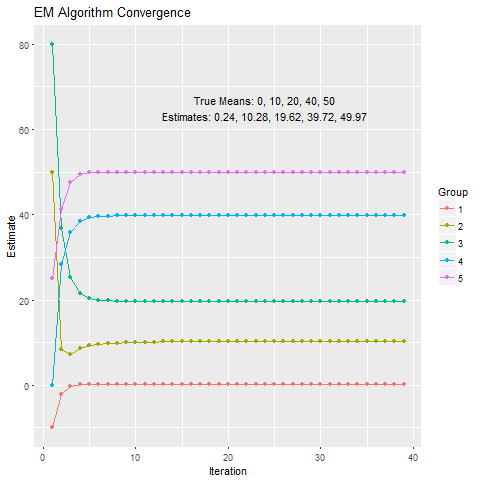
\includegraphics[width=0.8\linewidth]{EMconvergence-wonky}
\end{figure}
\end{frame}

%------------------------------------------------

\begin{frame}
\frametitle{Methodology}
"Conditional Sampling":
\begin{itemize}
\item Similar to the EM Algorithm, but instead of imputing the mean for the missing values, we draw random values from the distribution of the estimates of $\mu$ and $\Sigma$ for each iteration. The draws of values are then used to estimate the mean and covariance. (This method will not converge)

%This method is somewhat bayesian (just with uniform priors)

\end{itemize}
\medskip
% Conditional Normal Values:
\begin{equation*}
(\mathbf{x}_1 | \mathbf{x}_2=a) \sim N(\bar{\mu},\bar{\Sigma})
% \hat{\Sigma} = \frac{1}{N-1} \sum_{n=1}^N(x_n - \bar{x})(x_n - \bar{x})^\top
\end{equation*}

\begin{columns}[c] % The "c" option specifies centered vertical alignment while the "t" option is used for top vertical alignment

\column{.45\textwidth} % Left column and width
% \textbf{Mean Estimate (MLE)}
\begin{equation*}
\mathbf{\bar{\mu}} = \mathbf{\mu}_1 + \Sigma_{12}\Sigma_{22}^{-1}(a-\mu_{2})
% \hat{\Sigma} = \frac{1}{N-1} \sum_{n=1}^N(x_n - \bar{x})(x_n - \bar{x})^\top
\end{equation*}

\column{.5\textwidth} % Right column and width
% \textbf{ Covariance Estimate (Unbiased) }
\begin{equation*}
\bar{\Sigma} = \Sigma_{11} - \Sigma_{12}\Sigma_{22}^{-1}\Sigma_{21}
\end{equation*}

\end{columns}
\medskip
\medskip
\tiny{Note: subscript 1 refers to missing values, and subscript 2 refers to non-missing values}

\end{frame}



%------------------------------------------------

\begin{frame}
\frametitle{Table}
\begin{table}
\begin{tabular}{l l l}
\toprule
\textbf{Treatments} & \textbf{Response 1} & \textbf{Response 2}\\
\midrule
Treatment 1 & 0.0003262 & 0.562 \\
Treatment 2 & 0.0015681 & 0.910 \\
Treatment 3 & 0.0009271 & 0.296 \\
\bottomrule
\end{tabular}
\caption{Table caption}
\end{table}
\end{frame}

%------------------------------------------------
\section{Simulation Study}
%------------------------------------------------

%if I'm ready, then include them
%if not then maybe just talk about the methods

%------------------------------------------------
\section{Application}
%------------------------------------------------
\begin{frame}
\frametitle{Application}
We'll test these methods using data of characteristics of hepatitis patients:
\begin{table}[ht]
\centering
\begin{tabular}{rrrrrrr}
  \hline
 & Age & Bilirubin & AlkPhosphate & Sgot & AlbuMin & ProTime \\ 
  \hline
1 &  30 & 1.00 &  85 &  18 & 4.00 &  \\ 
  2 &  50 & 0.90 & 135 &  42 & 3.50 &  \\ 
  3 &  78 & 0.70 &  96 &  32 & 4.00 &  \\ 
  4 &  31 & 0.70 &  46 &  52 & 4.00 &  80 \\ 
  5 &  34 & 1.00 &  & 200 & 4.00 &  \\ 
  6 &  34 & 0.90 &  95 &  28 & 4.00 &  75 \\ 
   \hline
\end{tabular}
\end{table}
\end{frame}

\begin{frame}
\frametitle{Application}
\begin{table}[ht]
\centering
\begin{tabular}{rrrr}
  \hline
 & Throw Away & EM Algorithm & Conditional Sampling \\ 
  \hline
Age & 41.06 & 41.20 & 41.20 \\ 
  Bilirubin & 1.25 & 1.43 & 1.43 \\ 
  AlkPhosphate & 102.51 & 106.30 & 106.31 \\ 
  Sgot & 86.39 & 85.89 & 85.92 \\ 
  AlbuMin & 3.83 & 3.81 & 3.81 \\ 
  ProTime & 62.16 & 61.81 & 61.74 \\ 
   \hline
\end{tabular}
\end{table}

\end{frame}

%------------------------------------------------
\section{Conclusion}
%------------------------------------------------


\begin{frame}
\frametitle{Theorem}
\begin{theorem}[Mass--energy equivalence]
$E = mc^2$
\end{theorem}
\end{frame}

%------------------------------------------------

\begin{frame}[fragile] % Need to use the fragile option when verbatim is used in the slide
\frametitle{Verbatim}
\begin{example}[Theorem Slide Code]
\begin{verbatim}
\begin{frame}
\frametitle{Theorem}
\begin{theorem}[Mass--energy equivalence]
$E = mc^2$
\end{theorem}
\end{frame}\end{verbatim}
\end{example}
\end{frame}

%------------------------------------------------

\begin{frame}
\frametitle{Figure}
Uncomment the code on this slide to include your own image from the same directory as the template .TeX file.
%\begin{figure}
%\includegraphics[width=0.8\linewidth]{test}
%\end{figure}
\end{frame}

%------------------------------------------------

\begin{frame}[fragile] % Need to use the fragile option when verbatim is used in the slide
\frametitle{Citation}
An example of the \verb|\cite| command to cite within the presentation:\\~

This statement requires citation \cite{p1}.
\end{frame}

%------------------------------------------------

\begin{frame}
\frametitle{References}
\footnotesize{
\begin{thebibliography}{99} % Beamer does not support BibTeX so references must be inserted manually as below
\bibitem[Smith, 2012]{p1} John Smith (2012)
\newblock Title of the publication
\newblock \emph{Journal Name} 12(3), 45 -- 678.
\end{thebibliography}
}
\end{frame}

%------------------------------------------------

\begin{frame}
\Huge{\centerline{The End}}
\end{frame}

%----------------------------------------------------------------------------------------

\end{document}